\documentclass[11pt,a4paper,twocolumn]{article}
\usepackage[utf8]{inputenc}
\usepackage{amsmath}
\usepackage{amsfonts}
\usepackage{amssymb}
\usepackage{hyperref}
\usepackage{graphicx}
\usepackage{caption}
\usepackage{subcaption}
\usepackage[left=1in,right=1in,top=1in,bottom=1in]{geometry}
\author{Daniel Deutsch and Dan Crankshaw}
\title{Machine Learning: Final Paper}
\date{}
\begin{document}
\maketitle

\section{Introduction}

\section{Related Work}

\emph{Other Paper} \cite{feng2008hidden}

\section{The Algorithms and Data}

\subsection*{Data}

The data that will be used in the training and evaluation of the ANN and the HMM was gathered from
\href{http://ai.stanford.edu/~btaskar/ocr/}{an optical character recognition dataset from Stanford University}. The data is a collection of handwritten letters segemented from words in which all uppercase characters have been removed. We took the raw data and removed specific features included in the data that we intended not to use. The resulting data set is a list of binary pixel values of each character's 16 by 8 image.
\begin{figure}[h]
\centering
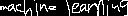
\includegraphics{img/ml.jpg}
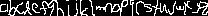
\includegraphics{img/alphabet.jpg}
\caption{An example of the data set}
\end{figure}

The data can often be difficult to read for a human. Figure 1 demonstrates this fact. Although it is possible to make out each letter, this task is made much easier by looking at the context of the word and anticipating what the letter should be. The figure also illustrates that many of the same letters are a variety of different sizes and are placed at different locations within the image. The quality of the data may make it difficult for the ANN to learn how to recognize each letter. However, the combination of the ANN and the HMM may be a good simulation of how a human would approach the problem: try to recognize the letter, then use context clues to figure out which character it is.

\subsection*{The Algorithms}

The two algorithms that we intend to use to accomplish the character recognition goal are an artificial neural network (ANN) and a hidden markov model (HMM). The idea is to compare the accuracy of the ANN to a combination of both the ANN and HMM to see if adding knowledge of word context to the model increases accuracy on the datasets.

The ANN will be trained on the pixel values for each letter image. Each training example is a 16 by 8 pixel image which amounts to an input size of 128. In order to help improve the accuracy of the classifier, we included a bias term on the input and hidden layers. Therefore, the input size for the ANN is 129 nodes.

Similarly, since we are trying to classify each image as a letter, there will need to be 26 output nodes, one for each lowercase letter in the alphabet. Therefore, the input and output sizes are set. The only parameters left to tune for the ANN are the number of hidden layers and the number of nodes within each hidden layer.

In order to find the best values for these parameters, we ran a series of tests on the development data set to try and tune the parameters. We compared the accuracies of each model on the development dataset to try and find the optimal parameters.

Each of the following tables was generated by randomly initializing an ANN with the given hidden layer sizes, then training them all on the same data. This process is repeated 10 times per data point, and the average accuracy is given.

For the ANN with one hidden layer, the only parameter than can be changed is the number of hidden nodes in that layer.
\begin{figure}[h]
\caption{Accuracies of two-layer networks}
\centering
\begin{tabular}{|c|c|}
\hline 
Hidden Nodes & Accuracy \\ 
\hline 
25 & • \\ 
\hline 
50 & • \\ 
\hline 
75 & • \\ 
\hline 
100 & • \\ 
\hline 
\end{tabular} 
\end{figure}

For the ANN with two hidden layers, the size of each hidden layer can be varied as well.

\begin{figure}[h]
\caption{Accuracies of three-layer networks}
\centering
\begin{tabular}{|c|c|c|}
\hline 
Layer 1 & Layer 2 & Accuracy \\ 
\hline 
50 & 25 & • \\ 
\hline 
50 & 50 & • \\ 
\hline 
100 & 25 & • \\ 
\hline 
100 & 50 & • \\ 
\hline 
100 & 100 & • \\ 
\hline 
\end{tabular} 

\end{figure}


\section{Results}

\section{Analysis}

\section{Conclusion}

\bibliography{refs.bib}
\bibliographystyle{plain}

\end{document}